%%%% ijcai15.tex

\typeout{Non-monotone Adaptive Submodular Maximization}

% These are the instructions for authors for IJCAI-15.
% They are the same as the ones for IJCAI-11 with superficical wording
%   changes only.

\documentclass{article}
% The file ijcai15.sty is the style file for IJCAI-15 (same as ijcai07.sty).
\usepackage{ijcai15}

% Use the postscript times font!
\usepackage{times}

% the following package is optional:
%\usepackage{latexsym} 

% Following comment is from ijcai97-submit.tex:
% The preparation of these files was supported by Schlumberger Palo Alto
% Research, AT\&T Bell Laboratories, and Morgan Kaufmann Publishers.
% Shirley Jowell, of Morgan Kaufmann Publishers, and Peter F.
% Patel-Schneider, of AT\&T Bell Laboratories collaborated on their
% preparation.

% These instructions can be modified and used in other conferences as long
% as credit to the authors and supporting agencies is retained, this notice
% is not changed, and further modification or reuse is not restricted.
% Neither Shirley Jowell nor Peter F. Patel-Schneider can be listed as
% contacts for providing assistance without their prior permission.

% To use for other conferences, change references to files and the
% conference appropriate and use other authors, contacts, publishers, and
% organizations.
% Also change the deadline and address for returning papers and the length and
% page charge instructions.
% Put where the files are available in the appropriate places.

%-------------------------------------------------------------------------------
% Custom definitions
%-------------------------------------------------------------------------------
\usepackage{etoolbox}
% Define output mode (default: six-page IJCAI)
\newtoggle{short}
\toggletrue{short}
% Uncomment for long version
%\togglefalse{short}

\usepackage[scaled=0.9]{inconsolata}
\usepackage[usenames,dvipsnames]{xcolor}
\usepackage{amsmath,amssymb,amsthm}
\usepackage{mathtools}                    % For \vcentcolon
\usepackage{xspace}                       % Controls space after user-defined command
\usepackage{xparse}                       % Optional arguments in commands
\usepackage{enumitem}
\usepackage{fixltx2e}                     % For subscripts in normal text
\usepackage{bm}
\usepackage{dsfont}                       % Indicator function (mathbb for numbers)
\usepackage{caption}
\usepackage{subcaption}
\usepackage{algorithm}
\usepackage{algorithmic}

\usepackage{tikz}
\usetikzlibrary{shapes,fit}
\usepackage{pgfplots}
\pgfplotsset{compat=newest}
\newlength\figureheight
\newlength\figurewidth

\iftoggle{short}
{
\usepackage{nohyperref}
\usepackage{url}
}
{
\usepackage{flushend}
\usepackage[debug]{hyperref}
\definecolor{mydarkblue}{rgb}{0,0.08,0.45}
\hypersetup{%
  pdftitle={Active Learning for Level Set Estimation},
  pdfauthor={},
  pdfsubject={},
  pdfkeywords={},
  pdfborder=0 0 0,
  pdfpagemode=UseNone,
  colorlinks=true,
  linkcolor=mydarkblue,
  citecolor=mydarkblue,
  filecolor=mydarkblue,
  urlcolor=mydarkblue,
  pdfview=FitH}
}

\newcommand{\todo}[1]{\noindent\texttt{\small\color[rgb]{0.5,0.1,0.1} TODO: #1}}

% Refs
\newcommand{\sectref}[1]{\hyperref[#1]{Section \ref*{#1}}}
\newcommand{\chapref}[1]{\hyperref[#1]{Chapter \ref*{#1}}}
\newcommand{\figref}[1]{\hyperref[#1]{Figure \ref*{#1}}}
\newcommand{\figsref}[1]{\hyperref[#1]{Figures \ref*{#1}}}
\newcommand{\tabref}[1]{\hyperref[#1]{ Table \ref*{#1}}}
\newcommand{\algoref}[1]{\hyperref[#1]{Algorithm \ref*{#1}}}
\newcommand{\theoremref}[1]{\hyperref[#1]{Theorem \ref*{#1}}}
\newcommand{\lemmaref}[1]{\hyperref[#1]{Lemma \ref*{#1}}}
\newcommand{\lemmasref}[1]{\hyperref[#1]{Lemmas \ref*{#1}}}
\newcommand{\corref}[1]{\hyperref[#1]{Corollary \ref*{#1}}}
\newcommand{\asref}[1]{\hyperref[#1]{Assumption \ref*{#1}}}
\newcommand{\eqtref}[1]{\hyperref[#1]{\mbox{(\ref*{#1})}}}
\newcommand{\appref}[1]{\hyperref[#1]{Appendix \ref*{#1}}}
\newcommand{\lineref}[1]{\hyperref[#1]{line \ref*{#1}}}
\newcommand{\linesref}[2]{\hyperref[#1]{lines \ref*{#1}--\ref*{#2}}}
\newcommand{\linsref}[1]{\hyperref[#1]{lines \ref*{#1}}}

% Theory environments
\newtheorem{definition}{Definition}
\newtheorem{theorem}{Theorem}
\newtheorem{lemma}{Lemma}
\newtheorem{cor}{Corollary}
\newtheorem{assumption}{Assumption}

% Algorithm-related
\newcommand{\theHalgorithm}{\arabic{algorithm}}
\renewcommand{\algorithmicrequire}{\textbf{Input:}}
\renewcommand{\algorithmicensure}{\textbf{Output:}}
\newcommand*\LNot{\textbf{not}\xspace}
\newcommand*\LAnd{\textbf{and}\xspace}
\newcommand*\LET[2]{\STATE #1 $\gets$ #2}
\newcommand*\Fcall[1]{\textsc{#1}}
\makeatletter
\newcommand{\setalglineno}[1]{%
  \setcounter{ALC@line}{\numexpr#1-1}}
\makeatother
\renewcommand{\algorithmiccomment}[1]{// #1}
\newcommand{\LINEIF}[2]{%
    \STATE\algorithmicif\ {#1}\ \algorithmicthen\ {#2}%
}
\newcommand{\LINEELSE}[1]{%
    \STATE\algorithmicelse\ {#1}%
}

% Math definitions
\newcommand{\argmax}{\operatornamewithlimits{argmax}}
\newcommand{\argmin}{\operatornamewithlimits{argmin}}
\def\*#1{\bm{#1}}

\newcommand{\twopartdef}[4]
{
	\left\{
		\begin{array}{ll}
			#1\,,& \mbox{if } #2 \\
			#3\,,& \mbox{if } #4
		\end{array}
	\right.
}

\newcommand{\twopartdefo}[3]
{
	\left\{
		\begin{array}{ll}
			#1\,,& \mbox{if } #2 \\
			#3\,,& \mbox{otherwise}
		\end{array}
	\right.
}

\newcommand{\defeq}{\vcentcolon=}

% Fix spacing problem with \left and \right
\let\originalleft\left
\let\originalright\right
\renewcommand{\left}{\mathopen{}\mathclose\bgroup\originalleft}
\renewcommand{\right}{\aftergroup\egroup\originalright}

% Math definitions
\newcommand{\smid}{\ \middle\vert\ }
\newcommand{\mmid}{\,\vert\,}

\DeclareDocumentCommand \E { o m o }{%
  \IfValueTF {#1} {%
    \mathbb{E}_{#1}
  }{%
    \mathbb{E}
  }%
  \left[#2
  \IfValueT {#3} {%
    \smid #3
  }%
  \right]
}

\DeclareDocumentCommand \P { o m o }{%
  \IfValueTF {#1} {%
    \mathbb{P}_{#1}
  }{%
    \mathbb{P}
  }%
  \left[#2
  \IfValueT {#3} {%
    \smid #3
  }%
  \right]
}

\newcommand{\D}[2]{\Delta(#1\mmid#2)}
\newcommand{\sdef}[2]{\left\{#1\smid#2\right\}}

\newcommand{\pio}{\pi_{[0]}}
\newcommand{\pii}{\pi_{[i]}}
\newcommand{\pik}{\pi_{[k]}}
\newcommand{\pis}{\pi^*}
\newcommand{\pisi}{\pi^*_{[i]}}
\newcommand{\pisk}{\pi^*_{[k]}}
\newcommand{\pigr}{\pi^{\textrm{g}}}
\newcommand{\pig}{\pi^{\textrm{rg}}}
\newcommand{\pigo}{\pi^{\textrm{rg}}_{[0]}}
\newcommand{\pigi}{\pi^{\textrm{rg}}_{[i]}}
\newcommand{\pigl}{\pi^{\textrm{rg}}_{[\ell]}}
\newcommand{\pigii}{\pi^{\textrm{rg}}_{[i+1]}}
\newcommand{\pigk}{\pi^{\textrm{rg}}_{[k]}}
\newcommand{\favg}{f_{\mathrm{avg}}}
\newcommand{\dom}{\mathcal{D}}
\newcommand{\Mk}{\mathcal{M}_k}

\newcommand{\uitem}[1]{\item[#1]}

% For citations like: Author et. al [2010]
\newcommand{\citet}[1]{\citeauthor{#1}~\shortcite{#1}}

% Paragraph
\renewcommand{\paragraph}[1]{\vspace{0.3em}\noindent\textbf{#1.}\makebox[0.5em]{}}

% Shortcuts
\newcommand{\fbook}{\textsc{Facebook}\xspace}
\newcommand{\gnutella}{\textsc{Gnuttela}\xspace}
\newcommand{\gplus}{\textsc{Google+}\xspace}
\newcommand{\twitter}{\textsc{Twitter}\xspace}
\newcommand{\infmax}{IM\xspace}
\newcommand{\maxcut}{MC\xspace}

\newcommand{\am}[1]{{\color{red!40!darkgray}\textbf{[Amin: #1]}}\xspace}
\newcommand{\ak}[1]{{\color{green!40!darkgray}\textbf{[AK: #1]}}\xspace}
%-------------------------------------------------------------------------------

\iftoggle{short}
{
\title{Non-monotone Adaptive Submodular Maximization}
}
{
\title{Non-monotone Adaptive Submodular Maximization\\\emph{\footnotesize (extended version with supplementary material)}}
}
%% \author{Alkis Gotovos\\
%% ETH Zurich
%% \And
%% Amin Karbasi\\
%% Yale University
%% \And
%% Andreas Krause\\
%% ETH Zurich}


\begin{document}

\maketitle

\begin{abstract}
A wide range of AI problems, such as sensor placement, active learning, and network influence maximization, require sequentially selecting elements from a large set with the goal of optimizing the utility of the selected subset.
Moreover, each element that is picked may provide stochastic feedback, which can be used to make smarter decisions about future selections.
Finding efficient policies for this general class of adaptive optimization problems can be extremely hard.
However, when the objective function is adaptive monotone and adaptive submodular, a simple greedy policy attains a $1-1/e$ approximation ratio in terms of expected utility.
Unfortunately, many practical objective functions are naturally non-monotone; to our knowledge, no existing policy has provable performance guarantees when the assumption of adaptive monotonicity is lifted.
We propose the \emph{adaptive random greedy policy} for maximizing adaptive submodular functions, and prove that it retains the aforementioned $1-1/e$ approximation ratio for functions that are also adaptive monotone, while it additionally provides a $1/e$ approximation ratio for non-monotone adaptive submodular functions.
We showcase the benefits of adaptivity on several network data sets using two non-monotone functions, representative of two classes of commonly encountered non-monotone objectives.
\end{abstract}

\section{Introduction}

Many practical problems in artificial intelligence boil down to selecting a number of elements from a large set of options in an initially unknown environment, so as to maximize some utility function defined over subsets of selected elements.
Example problems include sensor placement (selecting sensor locations), active learning (selecting examples to label), and network influence maximization (selecting seed nodes).
In contrast to the \emph{non-adaptive} setting, where we commit to the selected elements all at once, in the \emph{adaptive} setting the selection process is performed in a sequential manner, and each element that is picked provides some form of stochastic feedback, or, in other words, reveals part of the environment.
Naturally, we would like to leverage the acquired feedback to make smarter future selections.

\begin{figure}[tb]
  \centering
  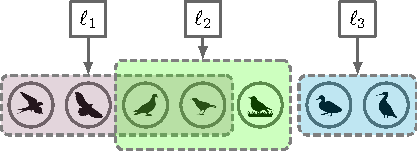
\includegraphics[width=0.4\textwidth]{figures/birdwatching.pdf}
  \caption{Birdwatching maximum cover example.}\label{fig:toy}
\end{figure}

As a running example, consider the toy instance of a stochastic maximum coverage problem shown in \figref{fig:toy}.
Suppose that square nodes represent birdwatching locations; by visiting each of them we observe a random number of bird species among those that are known to exist in that location.\footnote{\url{http://www.allaboutbirds.org/}}
We would like to plan a birdwatching trip to visit a number of these locations and maximize the number of observed species.
It is intuitive that taking into account the already observed species in deciding which place to visit next can be greatly beneficial compared to committing to the full trip in advance.

Since the general class of adaptive optimization problems in partially observable enviroments does not admit efficient policies, previous work has focused on characterizing subclasses of problems that can be solved efficiently.
Most notably, \citet{golovin11} showed that when the objective function under consideration is adaptive monotone and adaptive submodular, then a simple greedy policy attains a $1-1/e$ approximation ratio in terms of expected utility.

Adaptive submodularity and its intuitive meaning of ``diminishing returns'' is fundamental to a number of objective functions of interest in the adaptive setting.
However, the additional assumption of adaptive monotonicity, i.e., that adding an element to our selection always leads to an increase in expected utility, is often not satisfied in practice.
In our birdwatching example, the original objective is adaptive monotone submodular; however, if each subset of locations has an associated cost, e.g., the total required travel distance to visit all of them, our new objective will naturally be non-monotone.
More broadly, as we will see, a common way of obtaining adaptive submodular objectives is by generalizing non-adaptive submodular functions under certain assumptions about the form of stochastic feedback.
Despite the desire to generalize problems with non-monotone submodular objectives to the adaptive setting, no existing policies provide guarantees about non-monotone objectives in this setting.

To resolve this, we propose a new policy for maximizing non-monotone adaptive submodular functions, called \emph{adaptive random greedy}.
We prove that this policy retains the $1-1/e$ approximation ratio, if the function at hand is additionally adaptive monotone, while it also provides a $1/e$-approximation for non-monotone functions.
Our proposed policy generalizes the random greedy algorithm proposed by \citet{buchbinder14} for non-monotone submodular optimization to the adaptive setting.
We further discuss two common ways in which non-monotone adaptive submodular objectives come about, and present a representative example objective for each of them.
Finally, we evaluate our policy on these two objectives using a number of real-world network data sets, and, thereby, showcase the potential benefits of adaptivity.

\section{Problem Statement and Background}
Assume we are given a finite ground set $E$ and a set $O$ of observable states.
Each item $e \in E$ is associated with a state $o \in O$ through a function $\phi : E \to O$, which is called a \emph{realization} of the set of states.
We also assume that the realization $\Phi$ is a random variable with known distribution $p(\phi)$.
Furthermore, we are given an objective function $f : 2^E \times O^E \to \mathbb{R}_{\geq 0}$.
For a set $A \subseteq E$ and a realization $\phi$, the quantity $f(A, \phi)$ represents the utility of selecting subset $A$ when the true realization is $\phi$.
In our birdwatching example, the ground set $E$ consists of the three possible locations $\{\ell_1, \ell_2$, $\ell_3\}$ we may visit, and the state of each location is the (random) subset of bird species that we actually observe if we travel to that location; each realization maps all locations to subsets of actually observed species.
Our objective function is the total number of observed species given a subset of visited locations.

Our goal is to come up with a sequential policy that---initially unaware of $\phi$---builds up a set $A \subseteq E$, such that our utility $f(A, \phi)$ is maximized.
That is, we iteratively select an item $e \in E$ to add to $A$ and observe its state $\phi(e)$.
In this setting, there are two factors that complicate matters compared to its non-adaptive counterpart.
First, since utility depends on the random realization, the quantity of focus is the \emph{expected} utility under the distribution of realizations $p(\phi)$.
Second, the chosen set $A$ itself is a random variable that depends on the realization, since the choices of our policy will change according to each observation $\phi(e)$, which is, of course, the whole point of adaptivity.
In addition, the policy itself might make random decisions, which is an additional source of randomness for $A$.

To address the above complications, we define a \emph{partial realization} as a set $ \psi \subseteq E \times O$, which represents the item-observation pairs over a subset of $E$.
In particular, we call this subset the \emph{domain} of $\psi$, which is formally defined as $\dom(\psi) \defeq \sdef{e \in E}{\exists o \in O : (e, o) \in \psi}$.
Additionally, we write $\psi(e) = o$, if $(e, o) \in \psi$, and call $\psi$ \emph{consistent} with realization $\phi$ (denoted by $\phi \sim \psi$), if $\psi(e) = \phi(e)$, for all $e \in \dom(\psi)$, which means that the observations of a subset according to $\psi$ agree with the assignments over the whole ground set according to $\phi$.

We can now define a \emph{policy} $\pi$ as a function from partial realizations to a distribution $\mathcal{P}(E)$ over items that specifies which item to pick next, formally, $\pi : 2^{E \times O} \to \mathcal{P}(E)$. 
For birdwatching, our policy would specify which location to visit next (or, more generally, a distribution of next locations), given the already visited locations and the already observed species in each of them.
The policy terminates when the current partial realization is not in its domain denoted by $\dom(\pi) \subseteq 2^{E \times O}$.
We also use the shorthand notation $\pi(e\mmid\psi)$ for the probability of picking item $e$ given partial realization $\psi$.
We call $E(\pi, \phi) \subseteq E$ the set of items that have been selected upon termination of policy $\pi$ under realization $\phi$ (our final set of visited birdwatching locations).
Note that $E(\pi, \Phi)$ is a random variable that depends on both the randomness of the policy, as well as the randomness of realizations.

Finally, we can formally assess the performance of a policy $\pi$ via its expected utility,
\begin{align*}
  \favg(\pi) \defeq \E[\Phi,\Pi]{f(E(\pi, \Phi), \Phi)}.
\end{align*}
Then, our goal is to come up with a policy that maximizes the expected utility, subject to a cardinality constraint on the number of items to be picked, $|E(\pi, \Phi)| \leq k$.
In birdwatching terms, find a policy that maximizes the expected number of observed bird species, if we can visit at most $k$ locations.

\subsection{Monotonicity and Submodularity}
\paragraph{Non-adaptive}
Even in the non-adaptive setting, where we have to commit to a subset in advance, the problem of maximizing a set function $f : 2^E \to \mathbb{R}_{\geq 0}$, subject to a cardinality constraint $|A| \leq k$, is NP-hard in general.
In this setting, the marginal gain of an element $e \in E$ given set $B \subseteq E$ is defined as $f(B \cup \{e\}) - f(B)$.
Intuitively, the marginal gain quantifies the increase in utility if we add $e$ to our selection, given that we have already picked the elements in $B$.
Function $f$ is called \emph{monotone} if, for any $B \subseteq C \subseteq E$, it holds that $f(B) \leq f(C)$, which is equivalent to saying that the marginal gain is always non-negative.
Furthermore, $f$ is called \emph{submodular}, if, for any $B \subseteq C \subseteq E$ and any $e \in E \setminus C$, it holds that $f(C \cup \{e\}) - f(C) \leq  f(B \cup \{e\}) - f(B)$.
This means that the marginal gain of any element decreases as the given set increases ($C \supseteq B$); in other words, submodularity expresses a property of ``diminishing returns'' as more and more elements are added to our selection.

In their seminal work, \citet{nemhauser78} showed that, if $f$ is non-negative, monotone, and submodular, then constructing a subset $A$ of size $k$ by greedily picking elements according to their marginal gains, guarantees that $f(A)$ is a ($1 - 1/e$)-approximation of the optimal value.

\paragraph{Adaptive}
In the significantly more complex adaptive setting, the problem of computing an optimal policy is hard to approximate even for seemingly simple classes of objective functions (e.g., linear), as shown by \citet{golovin11}.
However, they also showed that the notions of monotonicity and submodularity can be naturally generalized to this setting, and lead to similar performance guarantees to the non-adaptive setting.

More concretely, the \emph{expected marginal gain} of an element $e \in E$ given partial realization $\psi$ can be defined as
\begin{align*}
  \D{e}{\psi} \defeq \E[\Phi]{f\big(\mathcal{D}(\psi) \cup \{e\}, \Phi\big) - f\big(\dom(\psi), \Phi\big)}[\Phi \sim \psi].
\end{align*}
The above expression is a conditional expectation, which only considers realizations that are consistent with $\psi$.
In birdwatching terms, it quantifies how many new species we expect to observe if we visit a new location $e$ given the already visited locations and already observed species in $\psi$.
Then, the following properties can be defined analogously to their non-adaptive counterparts:
\begin{itemize}
\item $f$ is called \emph{adaptive monotone}, if $\D{e}{\psi} \geq 0$, for all $e \in E$ and all $\psi$ of positive probability,
\item $f$ is called \emph{adaptive submodular}, if $\D{e}{\psi'} \leq \D{e}{\psi}$, for all $e \in E \setminus \dom(\psi')$ and all $\psi' \supseteq \psi$.
\end{itemize}

Given a number of previously selected elements and their corresponding observed states encoded in partial realization $\psi$, the adaptive greedy policy selects the element $e \in E \setminus \dom(\psi)$ of highest marginal gain $\D{e}{\psi}$, and continues to do so iteratively until $k$ elements have been selected.
\citet{golovin11} showed that, if $f$ is adaptive monotone submodular, then adaptive greedy is a $(1-1/e)$-approximation in terms of expected utility $\favg$.

\section{Adaptive Random Greedy}
While adaptive monotonicity is satisfied by many functions of interest, it is often the case that modeling practical problems naturally results in non-monotone objectives (see \sectref{sect:functions}); no existing policy provides provable performance gurantees in this case.
We now present our proposed adaptive random greedy policy ($\pig$) for maximizing adaptive submodular functions, and prove approximation ratios irrespective of whether adaptive monotonicity is satisfied or not.

For technical reasons that will become apparent below, let us assume that we always add a set $D$ of $2k - 1$ dummy elements to the ground set, such that, for any $d \in D$, and any partial realization $\psi$, it holds that $\D{d}{\psi} = 0$.
Obviously, these elements do not affect the optimal policy, and may be removed from the solution of any policy, without affecting its expected utility.

The detailed pseudocode of running the adaptive random greedy policy is presented \algoref{alg:rg}.
As discussed before, the algorithm is given a ground set and an objective function, as well as a known distribution over realizations $\Phi$.
At each iteration, the first step is to compute the expected marginal gain of each remaining element (\lineref{lin:marg}).
The key difference compared to the original adaptive greedy policy is shown in \linesref{lin:upd1}{lin:upd2}; rather than selecting the element with the largest expected marginal gain, $\pig$ randomly selects an element from the set $\Mk(\psi)$, which contains the elements with the $k$ largest gains.
The dummy elements added to the ground set ensure that the policy never picks an element with negative expected marginal gain.
Also, note that, although in \algoref{alg:rg} the returned set $A$ contains exactly $k$ elements, the actual selected set may very well contain less than $k$ elements, since we implicitly assume that any dummy elements are removed from it after the policy terminates.

When running the original adaptive greedy policy, non-monotonicity can lead to situations, where selecting the element of maximum marginal gain leads to traps of low utility that cannot be escaped.
In contrast, the randomization introduced by adaptive random greedy to the selection of each element helps dealing with such traps (on average) and, thus, leads to guaranteed approximation guarantees for the expected utility, even for non-monotone objectives.

\begin{algorithm}[tb]
  \caption{Adaptive random greedy}
  \label{alg:rg}
  \small{
    \begin{algorithmic}[1]
      \REQUIRE ground set $E$, function $f$, distribution $p(\phi)$, cardinality constraint $k$
      %  \ENSURE set $S_k \subseteq E$
      \LET{$A$}{$\varnothing$}
      \LET{$\psi$}{$\varnothing$}
      \FOR{$i = 1$ \TO $k$}
      \STATE Compute $\D{e}{\psi}$, for all $e \in E \setminus A$ \label{lin:marg}
      \LET{$\Mk(\psi)$}{$\displaystyle\argmax_{S \subseteq E \setminus A,\,|S| = k}\left\{\sum_{e \in S} \D{e}{\psi} \right\}$} \label{lin:upd1}
      \STATE Sample $m$ uniformly at random from $\Mk(\psi)$ \label{lin:upd2}
      \LET{$A$}{$A \cup \{m\}$}
      \STATE Observe $\Phi(m)$
      \LET{$\psi$}{$\psi \cup \left\{\big(m, \Phi(m)\big)\right\}$}
      \ENDFOR
      \STATE Return $A$
    \end{algorithmic}
  }
\end{algorithm}

\paragraph{Theoretical analysis}
More concretely, we now show that the adaptive random greedy policy retains the $1-1/e$ approximation ratio for adaptive monotone submodular objectives, while, at the same time, it achieves a $1/e$ approximation ratio for non-monotone objectives, under the additional condition of submodularity for each realization.
As we will see in \sectref{sect:functions}, for the vast majority of non-monotone objectives used in practice this condition holds by way of construction.
We, therefore, do not consider it a major restriction in the choice of objectives.
Our proofs generalize the results of \citet{buchbinder14} for the random greedy algorithm, and are presented in detail in the long version of this paper;\footnote{\url{http://sites.google.com/site/nonmonijcai15/long.pdf}} in what follows, we provide an outline of our analysis.

First, let us define the expected gain of running policy $\pi$ after having obtained a partial realization $\psi$, as
{\small
\begin{align*}
  \D{\pi}{\psi} \defeq \E[\Phi,\Pi]{f(\dom(\psi) \cup E(\pi, \Phi), \Phi) - f(\dom(\psi), \Phi)}[\Phi \sim \psi].
\end{align*}}
Also, for any policy $\pi$ and any positive integer $k$, we define the truncated policy $\pik$, which runs indentically to $\pi$ for $k$ steps and then terminates.
Finally, given any two policies $\pi_1$, $\pi_2$, we denote by $\pi_1@\pi_2$ the policy that first runs $\pi_1$ until it terminates and then runs $\pi_2$, discarding all observations made by $\pi_1$.
After $\pi_1@\pi_2$ terminates, the subset selected by it consists of the union of the subsets selected by each policy individually.

The following is a key lemma for both monotone and non-monotone objectives.
\setcounter{lemma}{0}
\begin{lemma}\label{lem:submod}
  If $f$ is adaptive submodular, then, for any policy $\pi$, and any partial realization $\psi$, it holds that
  \begin{align*}
    \D{\pik}{\psi} \leq \sum_{e \in \Mk(\psi)} \D{e}{\psi}.
  \end{align*}
\end{lemma}
\noindent It states the intuitive fact that, at any point, no $k$-step policy can give us a larger expected gain than the sum of the $k$ currently largest expected marginal gains.
This is a consequence of adaptive submodularity, which guaratees that the expected marginal gains of any element will decrease as our selection grows larger.

Based on \lemmaref{lem:submod} and the fact that $\pig$ selects at each step one of the $k$ elements in $\Mk$ uniformly at random, we can show the following lemma, which also applies to both monotone and non-monotone objectives.
\begin{lemma}\label{lem:mon_main}
  For any policy $\pi$, and any non-negative integer $i < k$, if $f$ is adaptive submodular, then
  \begin{align*}
    \favg(\pigii) - \favg(\pigi) \geq \frac{1}{k}\left(\favg(\pigi @ \pi) - \favg(\pigi)\right).
  \end{align*}
\end{lemma}
\noindent The lemma compares the expected gain at the $i$-th step of $\pig$ to the total gain of running any other policy (e.g., the optimal one) after the $i$-th step and, thereby, provides a means for obtaining approximation guarantees for $\pig$, as long as we can bound the term $\favg(\pigi @ \pi)$.
The dichotomy between adaptive monotone and non-monotone objectives in terms of theoretical guarantees stems from the different approaches in bounding this term.

If $f$ is adaptive monotone, we may use the trivial bound $\favg(\pigi @ \pi) \geq \favg(\pi)$, which follows from the definition of adaptive monotonicity, to obtain the following theorem.
\begin{theorem}
  If $f$ is adaptive monotone submodular, then for any policy $\pi$, and all integers $i, k > 0$ it holds that
  \begin{align*}
    \favg(\pigi) \geq \left(1 - e^{-i/k}\right)\favg(\pik).
  \end{align*}
\end{theorem}
\noindent In particular, by setting $i = k$ we get the familiar $1-1/e$ approximation ratio for $\pigk$.

For the non-monotone case, we need to leverage the randomness of the selection process of $\pig$ to bound $\favg(\pigi @ \pi)$.
For that purpose, we generalize to the adaptive setting the following lemma shown by \citet{buchbinder14}, which itself is based on a lemma by \citet{feige07} for the expected value of a submodular function under a randomly selected subset.
\begin{lemma}[\cite{buchbinder14}]
  If $f : 2^E \to \mathbb{R}_{\geq 0}$ is submodular and $A$ is a random subset of $E$, such that each element $e \in E$ is contained in $A$ with probability at most $p$, that is, $\P[A]{e \in A} \leq p,\ \forall e \in E$, then
  \begin{align*}
    \E[A]{f(A)} \geq (1-p)f(\varnothing).
  \end{align*}
\end{lemma}
\noindent Roughly speaking, the lemma states that a ``random enough'' subset $A$ cannot have much worse value than that of the empty set.
Note that $f$ is not assumed to be monotone here.

The following lemma extends the above claim to the adaptive setting.
\begin{lemma}
  If $f$ is adaptive submodular, and, additionally, $f(\cdot\,, \phi) : 2^E \to \mathbb{R}_{\geq 0}$ is submodular for all $\phi \in O^E$, then for any policy $\pi$ such that each element of $e \in E$ is selected by it with probability at most $p$, that is, $\P[\Pi]{e \in E(\pi, \phi)} \leq p,\ \forall \phi \in O^E,\ \forall e \in E$, the expected value of running $\pi$ can be bounded as follows:
\begin{align*}
  \favg(\pi) \geq (1-p)\,\favg(\pio).
\end{align*}
\end{lemma}
%\noindent Although we have not found concrete examples of adaptive submodular functions that do not satisfy this lemma, adaptive submodularity by itself does not seem to be a sufficient condition for it to hold; rather, we require the additional assumption that $f$ be submodular in its first argument for any realization.

As a consequence of the above lemma, we get that $\favg(\pigi@\pi) = \favg(\pi@\pigi) \geq (1-p)\favg(\pi)$, i.e., the elements added by adaptive random greedy cannot dramatically reduce the average value obtained by any other policy $\pi$.
Here, the probability $p$ can be bounded by using the fact that $\pig$ randomly selects one of $k$ elements at each step, hence at the $i$-step we have $p \leq (1-1/k)^i$.
Putting it all together, we obtain our main theorem for non-monotone objectives.
\begin{theorem}\label{thm:nonm}
  If $f$ is adaptive submodular, and $f(\cdot\,, \phi) : 2^E \to \mathbb{R}_{\geq 0}$ is submodular for all $\phi \in O^E$, then, for any policy $\pi$, and all integers $i, k > 0$, it holds that
  \begin{align*}
    \favg(\pigi) \geq \frac{i}{k}\left(1 - \frac{1}{k}\right)^{i-1}\favg(\pik).
  \end{align*}
\end{theorem}
\noindent By setting $i = k$, we get a $1/e$ approximation ratio for $\pigk$.

\section{Examples of Non-Monotone Objectives} \label{sect:functions}
To underline the importance of non-monotonicity, we now present two different ways, in which non-monotone adaptive submodular functions commonly arise in practice.
Both of the resulting classes of functions satisfy the assumptions of \theoremref{thm:nonm}, and are, therefore, suitable to be maximized using adaptive random greedy.
We also introduce two representative example objectives, one for each class, which are themselves of practical interest.

\subsection{Objectives with a Modular Cost Term}
Assume we are given an adaptive monotone submodular function $f_{\textrm{utility}}(A, \phi)$.
In practice, apart from benefit, there might also be some associated cost with the selection of each element, which can be directly incorporated into the objective function via a modular cost term a cost term $f_{\textrm{cost}}(A) = \sum_{a \in A} c_a$.
In this case, the resulting objective is of the form
\begin{align} \label{eq:cost}
  f(A, \phi) = f_{\textrm{utility}}(A, \phi) - f_{\textrm{cost}}(A),
\end{align}
which is also adaptive submodular, but non-monotone.

A common alternative to the above is to introduce a knapsack constraint $f_{\textrm{cost}}(A) \leq C$, while retaining a monotone objective.
Choosing a budget $C$, in this case, might not be obvious, whereas the formulation of equation \eqref{eq:cost} is often more straightforward, particularly when $f_{\textrm{cost}}$ is expressed in the same units as $f_{\textrm{utility}}$.

\paragraph{Influence maximization}
The concept of influence maximization in a social network was posed by \citet{kempe03} and has direct applications to problems such as viral marketing.
Given a graph and a model of influence propagation, the goal is to select a subset of nodes that are initially active, in order to maximize the spread of influence measured by the expected number of nodes that will ultimately be active according to the propagation model.
We focus here on the independent cascade model, according to which, each edge of the graph is randomly either ``live'' or ``blocked'', independently of any other edge in the network, and influence can only flow along ``live'' edges.

For this problem, the ground set $E$ consists of network nodes, and each realization $\phi$ corresponds to a full outcome of the independent cascade model, that is, an assignment to each network edge of being either ``live'' or ``blocked''.
The objective $f_{\textrm{inf}}(A, \phi)$ is the number of ultimately active nodes under realization $\phi$, if the nodes in the selected subset $A$ are initially active.
In the adaptive version of the problem, when a node $v$ is selected, it reveals the status (``live'' or ``blocked'') of all outgoing edges of $v$ and of any other node that can be reached from $v$ through ``live'' edges.
\citet{kempe03} showed that $f_{\textrm{inf}}$ is non-negative, monotone, and submodular, for any realization $\phi$; \citet{golovin11} showed that it is also adaptive monotone submodular.

Now, assume that each selected node incurs a unit cost, that is, we have a cost term $f_{\textrm{cost}}(A) = |A|$, which results in the following objective:
\begin{align*}
  \tilde{f}_{\textrm{inf}}(A, \Phi) \defeq f_{\textrm{inf}}(A, \Phi) - |A|.
\end{align*}
Since our cost term is modular, $\tilde{f}_{\textrm{inf}}$ has the form of equation \eqref{eq:cost}, and, therefore, is non-monotone adaptive submodular.
It is also non-negative, since $f_{\textrm{inf}}(A, \Phi) \geq |A|$.

\subsection{Objectives with Factorial Realizations}
Assume we are given a utility function $f(A, \phi)$, whose dependence of $\phi$ is constrained to the outcomes of the selected elements.
More formally, there exists a function $g : 2^{E \times O} \to \mathbb{R}_{\geq 0}$, such that $f(A, \phi) = g\left(\{(e, \phi(e)) \mid e \in A\}\right)$.
Furthermore, assume that $f$ is submodular in its first argument, for any realization $\phi$, and that the distribution of realizations factorizes over the elements of the ground set $E$, that is, $\P[\Phi]{\phi} = \prod_{e \in E}\P[\Phi(e)]{\phi(e)}$.
Given the above assumptions, it follows that $f$ is adaptive submodular (see Theorem 6.1 of \citet{golovin11}).

\paragraph{Maximum graph cut}
The problem of finding the maximum cut in a graph $(\mathcal{V}, \mathcal{E})$ has the following objective:
\begin{align*}
  f_{\textrm{cut}}(A) = \sum_{(v, w) \in \mathcal{E}} \mathds{1}_{\left\{v \in A, w \in \mathcal{V}\setminus A\ \textrm{or}\ v \in \mathcal{V}\setminus A, w \in A\right\}},
\end{align*}
which is non-negative and submodular.
Furthermore, it is symmetric, i.e., $f(A) = f(\mathcal{V}\setminus A)$, which implies that it is also non-monotone.
We consider here an adaptive version of the maximum cut problem, where the selection of a node triggers either cutting that node itself, or a random neighbor of it with some prespecified probability.

Again, the ground set $E$ consists of network nodes, and each realization $\phi$ corresponds to a function $\sigma_{\phi}$ that maps each node $v \in V$ to the node that would actually be cut, were $v$ to be selected.
Our adaptive max-cut objective can then be written as follows:
\begin{align*}
  \tilde{f}_{\textrm{cut}}(A, \Phi) \defeq f_{\textrm{cut}}\left(\bigcup_{v \in A}\sigma_{\Phi}(v)\right).
\end{align*}
We can directly see that, in terms of the realization $\Phi$, $\tilde{f}_{\textrm{cut}}$ only depends on the outcomes of the selected elements.
Furthermore, the distribution of realizations is factorial, since the outcome of each node cut is independent of all the others, i.e., $\sigma_{\phi}(v) = \hat{\sigma}_{\phi(v)}(v)$.
Finally, since $f_{\textrm{cut}}$ is submodular, it follows that $\tilde{f}_{\textrm{cut}}$ is submodular in its first argument for any realization.
We conclude that $\tilde{f}_{\textrm{cut}}$ satisfies the properties described above, hence it is (non-monotone) adaptive submodular.
It is also non-negative, because $f_{\textrm{cut}}$ is non-negative.

\section{Experiments}
We have evaluated our proposed algorithm on the two objective functions, namely influence maximization, and maximum cut, described in the previous section on several real-world data sets.
Since we have no competitor policy for the adaptive non-monotone submodular setting, we rather focus here on showcasing the potential benefits of adaptivity by comparing adaptive to non-adaptive random greedy.

\subsection{Data Sets and Experimental Setup}
For our experiments, we used $10$ networks from the KONECT\footnote{\url{http://konect.uni-koblenz.de/}} database, which accumulates network data sets from various other sources.
The network sizes range from a few thousands to tens of thousands nodes.

Computing the (expected) marginal gains is at the heart of both the non-adaptive random greedy algorithm and our proposed adaptive random greedy policy.
In terms of computational complexity, this may range from being completely straightforward to extremely demanding, depending on the specific objective at hand.
For the influence optimization objective, the exact computation of the expected influence of a subset of nodes has been shown to be NP-hard \cite{kempe03}.
To obtain an estimate we use Monte Carlo sampling over the outcomes of the independent cascades.
Note that within adaptive random greedy we have to perform this simulation at every step, while conditioning on the observations obtained up to that step.
For the maximum cut objective, it is very simple to compute the marginal gains in the adaptive case, since we already know at each step the outcomes of the previously selected nodes.
In the non-adaptive setting, however, this is considerably harder, since we have to average over every possible outcome of the current selection; we again resort to sampling from the space of possible realizations to obtain estimates.
To make the aforementioned computations more efficient, we subsample each network down to $2000$ nodes, using a technique based on random walks proposed by \citet{leskovec06}.

For both objectives, we select uniformly at random a subset of $100$ nodes as the ground set $E$, and repeat the experiments for $50$ such sets.
For each ground set instance, we evaluate the algorithms' performance on $100$ random realizations.

\setlength\figureheight{0.205\textwidth}
\setlength\figurewidth{0.29\textwidth}
\newcommand{\subflen}{0.245\textwidth}
\newcommand{\scspacey}{-1.8em}
\newcommand{\scspacex}{0.2em}
\begin{figure*}[tb]
  \captionsetup[subfigure]{oneside,margin={2em,0em}}
  \begin{subfigure}[b]{\subflen}
    \centering
    \begin{tikzpicture}

\begin{axis}[%
tick label style={font=\scriptsize},
label style={font=\scriptsize},
legend style={font=\scriptsize},
view={0}{90},
width=\figurewidth,
height=\figureheight,
xmin=0, xmax=100,
xtick={0, 20, 40, 60, 80, 100},
xlabel={$k$},
xlabel shift=-0.7em,
ymin=0, ymax=25,
ylabel={$\%$ imp.},
ylabel shift=-0.7em,
tick label style={/pgf/number format/fixed},
major tick length=2pt,
axis lines*=left,
legend cell align=left,
clip=true]

\addplot [
mark=*,
mark size=1.7pt,
color=cyan!60!black,
line width=1.3pt,
error bars/.cd,
error bar style={line width=1pt},
y dir=both,
y explicit
]
coordinates{
(1,-1.26492981839)+- (2*5.19525612056,2*5.19525612056)(10,4.84994554964)+- (2*3.32759806783,2*3.32759806783)(30,13.2044368445)+- (2*1.52581029456,2*1.52581029456)(50,9.68624070106)+- (2*0.521013033356,2*0.521013033356)(70,5.48852332314)+- (2*0.520732435039,2*0.520732435039)(100,4.00174517241)+- (2*0.195865078159,2*0.195865078159)
};

\end{axis}
\end{tikzpicture}

    \vspace{\scspacey}
    \caption{\hspace{\scspacex}\infmax{} -- \fbook}
    \label{fig:inf_ego_fb}
  \end{subfigure}
  \begin{subfigure}[b]{\subflen}
    \begin{tikzpicture}

\begin{axis}[%
tick label style={font=\scriptsize},
label style={font=\scriptsize},
legend style={font=\scriptsize},
view={0}{90},
width=\figurewidth,
height=\figureheight,
xmin=0, xmax=100,
xtick={0, 20, 40, 60, 80, 100},
xlabel={$k$},
xlabel shift=-0.7em,
ymin=0, ymax=25,
ylabel={$\%$ imp.},
ylabel shift=-0.7em,
tick label style={/pgf/number format/fixed},
major tick length=2pt,
axis lines*=left,
legend cell align=left,
clip=true]

\addplot [
mark=*,
mark size=1.5pt,
color=green!70!black,
line width=1pt,
error bars/.cd,
error bar style={line width=1pt},
y dir=both,
y explicit
]
coordinates{
(1,-2.99755271966)+- (2*4.49248359081,2*4.49248359081)(10,2.92935605827)+- (2*0.846305087059,2*0.846305087059)(30,2.50393369837)+- (2*0.138026001685,2*0.138026001685)(50,2.15500865653)+- (2*0.19618878656,2*0.19618878656)(70,2.53966691782)+- (2*0.169732149982,2*0.169732149982)(100,2.27364939629)+- (2*0.0941777497952,2*0.0941777497952)
};

\end{axis}
\end{tikzpicture}

    \vspace{\scspacey}
    \caption{\hspace{\scspacex}\infmax{} -- \gplus}
    \label{fig:inf_gplus}
  \end{subfigure}
  \begin{subfigure}[b]{\subflen}
    \begin{tikzpicture}

\begin{axis}[%
tick label style={font=\scriptsize},
label style={font=\scriptsize},
legend style={font=\scriptsize},
view={0}{90},
width=\figurewidth,
height=\figureheight,
xmin=0, xmax=100,
xtick={0, 20, 40, 60, 80, 100},
xlabel={$k$},
xlabel shift=-0.7em,
ymin=-5, ymax=20,
ytick={-5, 10, 20},
ylabel={$\%$ imp.},
ylabel shift=-0.7em,
tick label style={/pgf/number format/fixed},
major tick length=2pt,
axis lines*=left,
legend cell align=left,
clip=false]

\addplot [
  dashed,
  gray,
  line width=0.7pt
]
coordinates{
(0,0)(100,0)
};

\addplot [
mark=*,
mark size=1.7pt,
color=cyan!60!black,
line width=1.3pt,
error bars/.cd,
error bar style={line width=1pt},
y dir=both,
y explicit
]
coordinates{
(1,0.696522489083)+- (2*3.03413358384,2*3.03413358384)(10,7.85355180893)+- (2*1.55428481286,2*1.55428481286)(30,5.56795703127)+- (2*0.501794416201,2*0.501794416201)(50,6.96889887354)+- (2*0.807792478119,2*0.807792478119)(70,8.76175623121)+- (2*0.571860090691,2*0.571860090691)(100,3.4993021708)+- (2*0.0982055482729,2*0.0982055482729)
};

\end{axis}
\end{tikzpicture}

    \vspace{\scspacey}
    \caption{\hspace{\scspacex}\infmax{} -- \twitter}
    \label{fig:inf_twitter}
  \end{subfigure}
  \begin{subfigure}[b]{\subflen}
    \begin{tikzpicture}

\begin{axis}[%
tick label style={font=\scriptsize},
label style={font=\scriptsize},
legend style={font=\scriptsize},
view={0}{90},
width=\figurewidth,
height=\figureheight,
xmin=0, xmax=1,
xtick={0, 0.2, 0.4, 0.6, 0.8, 1},
xlabel={$p$},
xlabel shift=-0.7em,
ymin=0, ymax=25,
ylabel={$\%$ imp.},
ylabel shift=-0.7em,
tick label style={/pgf/number format/fixed},
major tick length=2pt,
axis lines*=left,
legend cell align=left,
clip=true]

\addplot [
mark=*,
mark size=1.7pt,
color=orange!70!black,
line width=1.3pt,
error bars/.cd,
error bar style={line width=1pt},
y dir=both,
y explicit
]
coordinates{
(0.1,21.347649113)+- (2*2.09964023732,2*2.09964023732)(0.3,5.75788402373)+- (2*0.739715175267,2*0.739715175267)(0.5,1.24762060304)+- (2*0.133082830759,2*0.133082830759)(0.75,0.285865475355)+- (2*0.0122944911964,2*0.0122944911964)(1.0,0.0)+- (2*0.0,2*0.0)
};

\end{axis}
\end{tikzpicture}

    \vspace{\scspacey}
    \caption{\hspace{\scspacex}\infmax{} -- \fbook}
    \label{fig:pinf_ego_fb}
  \end{subfigure}\\[0.5em]
  \begin{subfigure}[b]{\subflen}
    \begin{tikzpicture}

\begin{axis}[%
tick label style={font=\scriptsize},
label style={font=\scriptsize},
legend style={font=\scriptsize},
view={0}{90},
width=\figurewidth,
height=\figureheight,
xmin=0, xmax=50,
xtick={0, 10, 20, 30, 40, 50},
xlabel={$k$},
xlabel shift=-0.5em,
ymin=0, ymax=0.953648309179,
ylabel={$f_{\textrm{avg}}$},
ylabel shift=-0.5em,
tick label style={/pgf/number format/fixed},
major tick length=2pt,
axis lines*=left,
legend cell align=left,
clip=false]

\addplot [
mark=*,
mark size=1.5pt,
color=green!70!black,
line width=1pt,
error bars/.cd,
error bar style={line width=1pt},
y dir=both,
y explicit
]
coordinates{
(1,0.104346859903)+- (2*0.0168383469436,2*0.0168383469436)(5,0.39914589372)+- (2*0.0169434020126,2*0.0169434020126)(15,0.740953623188)+- (2*0.0199980710895,2*0.0199980710895)(25,0.831012560386)+- (2*0.0111356508511,2*0.0111356508511)(35,0.917506280193)+- (2*0.00654704276419,2*0.00654704276419)(50,0.932712077295)+- (2*0.0080656076662,2*0.0080656076662)
};

\addplot [
mark=*,
mark size=1.5pt,
color=orange!70!black,
line width=1pt,
error bars/.cd,
error bar style={line width=1pt},
y dir=both,
y explicit
]
coordinates{
(1,0.169610628019)+- (2*0.00547188956327,2*0.00547188956327)(5,0.495463768116)+- (2*0.00596831689451,2*0.00596831689451)(15,0.790107246377)+- (2*0.00716778696454,2*0.00716778696454)(25,0.882191304348)+- (2*0.010042521912,2*0.010042521912)(35,0.9236647343)+- (2*0.00516532222278,2*0.00516532222278)(50,0.904314009662)+- (2*0.0123394857599,2*0.0123394857599)
};

\addplot [
mark=*,
mark size=1.5pt,
color=cyan!70!black,
line width=1pt,
error bars/.cd,
error bar style={line width=1pt},
y dir=both,
y explicit
]
coordinates{
(1,0.169610628019)+- (2*0.00547188956327,2*0.00547188956327)(5,0.616156521739)+- (2*0.00678539557648,2*0.00678539557648)(15,0.932752657005)+- (2*0.00565679012947,2*0.00565679012947)(25,0.940901449275)+- (2*0.00914238321022,2*0.00914238321022)(35,0.953648309179)+- (2*0.00656270976912,2*0.00656270976912)(50,0.941888888889)+- (2*0.0079743861995,2*0.0079743861995)
};

\end{axis}
\end{tikzpicture}

    \vspace{\scspacey}
    \caption{\hspace{\scspacex}\maxcut{} -- \fbook}
    \label{fig:mc_ego_fb}
  \end{subfigure}
  \begin{subfigure}[b]{\subflen}
    \begin{tikzpicture}

\begin{axis}[%
tick label style={font=\scriptsize},
label style={font=\scriptsize},
legend style={font=\scriptsize},
view={0}{90},
width=\figurewidth,
height=\figureheight,
xmin=0, xmax=100,
xtick={0, 20, 40, 60, 80, 100},
xlabel={$k$},
xlabel shift=-0.7em,
ymin=0, ymax=25,
ylabel={$\%$ imp.},
ylabel shift=-0.7em,
tick label style={/pgf/number format/fixed},
major tick length=2pt,
axis lines*=left,
legend cell align=left,
clip=true]

\addplot [
mark=*,
mark size=1.5pt,
color=green!70!black,
line width=1pt,
error bars/.cd,
error bar style={line width=1pt},
y dir=both,
y explicit
]
coordinates{
(1,0.0)+- (2*0.0,2*0.0)(10,10.8357457973)+- (2*0.521973973886,2*0.521973973886)(30,9.16874203696)+- (2*0.354659968468,2*0.354659968468)(50,7.34755265405)+- (2*0.440275866343,2*0.440275866343)(70,9.44757194759)+- (2*0.440117769203,2*0.440117769203)(100,0.897599846484)+- (2*0.0939462561521,2*0.0939462561521)
};

\end{axis}
\end{tikzpicture}

    \vspace{\scspacey}
    \caption{\hspace{\scspacex}\maxcut{} -- \gplus}
    \label{fig:mc_gplus}
  \end{subfigure}
  \begin{subfigure}[b]{\subflen}
    \begin{tikzpicture}

\begin{axis}[%
tick label style={font=\scriptsize},
label style={font=\scriptsize},
legend style={font=\scriptsize},
view={0}{90},
width=\figurewidth,
height=\figureheight,
xmin=1, xmax=100,
xtick={1, 20, 40, 60, 80, 100},
xlabel={$k$},
xlabel shift=-0.7em,
ymin=-5, ymax=20,
ytick={-5, 10, 20},
ylabel={$\%$ imp.},
ylabel shift=-0.7em,
tick label style={/pgf/number format/fixed},
major tick length=2pt,
axis lines*=left,
legend cell align=left,
clip=false]

\addplot [
  dashed,
  gray,
  line width=0.7pt
]
coordinates{
(0,0)(100,0)
};

\addplot [
mark=*,
mark size=1.7pt,
color=cyan!60!black,
line width=1.3pt,
error bars/.cd,
error bar style={line width=1pt},
y dir=both,
y explicit
]
coordinates{
(1,0.0)+- (2*0.0,2*0.0)(2,6.9040513628)+- (2*1.14364309785,2*1.14364309785)(5,9.48924659278)+- (2*1.1598543596,2*1.1598543596)(10,8.32513052818)+- (2*0.643518509977,2*0.643518509977)(15,8.23839582147)+- (2*0.579625508212,2*0.579625508212)(20,6.82258618825)+- (2*0.630226068313,2*0.630226068313)(30,6.19886061482)+- (2*0.584787894761,2*0.584787894761)(40,4.8558088865)+- (2*0.632749095704,2*0.632749095704)(60,3.59181871414)+- (2*0.854178595527,2*0.854178595527)(80,5.38906765656)+- (2*0.485875191957,2*0.485875191957)(100,1.8825691516)+- (2*0.222526928393,2*0.222526928393)
};

\end{axis}
\end{tikzpicture}

    \vspace{\scspacey}
    \caption{\hspace{\scspacex}\maxcut{} -- \twitter}
    \label{fig:mc_twitter}
  \end{subfigure}
  \begin{subfigure}[b]{\subflen}
    \begin{tikzpicture}

\begin{axis}[%
tick label style={font=\scriptsize},
label style={font=\scriptsize},
legend style={font=\scriptsize},
view={0}{90},
width=\figurewidth,
height=\figureheight,
xmin=0, xmax=1,
xtick={0, 0.2, 0.4, 0.6, 0.8, 1},
xlabel={$\beta$},
xlabel shift=-0.7em,
ymin=0, ymax=25,
ylabel={$\%$ imp.},
ylabel shift=-0.7em,
tick label style={/pgf/number format/fixed},
major tick length=2pt,
axis lines*=left,
legend cell align=left,
clip=true]

\addplot [
mark=*,
mark size=1.7pt,
color=orange!70!black,
line width=1.3pt,
error bars/.cd,
error bar style={line width=1pt},
y dir=both,
y explicit
]
coordinates{
(0.0,5.13812950589)+- (2*0.573233591808,2*0.573233591808)(0.2,5.16884873742)+- (2*0.631370403375,2*0.631370403375)(0.4,4.2050408687)+- (2*0.612632341345,2*0.612632341345)(0.6,2.58737479526)+- (2*0.907094746934,2*0.907094746934)(0.8,2.32418126481)+- (2*1.59527432864,2*1.59527432864)(1.0,0.51104313314)+- (2*2.39915042051,2*2.39915042051)
};

\end{axis}
\end{tikzpicture}

    \vspace{\scspacey}
    \caption{\hspace{\scspacex}\maxcut{} -- \twitter}
    \label{fig:pmc_twitter}
  \end{subfigure}
  \vspace{-0.2em}
  \caption{
    Improvement in expected utiliy of using adaptive vs. non-adaptive random greedy.
    Top: influence maximization; \emph{(a)--(c)} improvement vs. node budget $k$; \emph{(d)} improvement vs. independent cascade edge probability $p$.
    Bottom: maximum cut; \emph{(e)--(g)} improvement vs. node budget $k$; \emph{(h)} improvement vs. cut distribution parameter $\beta$.
  }
  \label{fig:exp}
\end{figure*}

\subsection{Results}
We present here results for three of the network data sets, which are ego networks from Facebook, Google+, and Twitter respectively \cite{mcauley12}.
\figref{fig:exp} shows the $\%$ relative improvement of adaptive random greedy over its non-adaptive counterpart in terms of expected utility for influence maximization (top) and maximum cut (bottom).
In the first three figures of each row, we plot the improvement for different values of the cardinality constraint $k$.
For the influence maximization objective, the influence propagation probability of each edge is chosen to be $p=0.1$, and for the maximum cut objective, selecting a node cuts itself or one of its neighbors with equal probability.

We can see that adaptivity is beneficial in general, while the improvement it provides varies substantially depending on the properties of each network.
As an example, for networks containing a few nodes of very high degree, like the Google+ network in plots (c) and (g), adaptivity provides little benefit for influence maximization, since these nodes are the main source of influence, hence are almost always selected by the non-adaptive algorithm as well.
On the other hand, adaptivity is much more beneficial for the maximum cut objective in such networks, since the feedback of whether such high degree nodes have already been cut by some of their neighbors helps making future selections more efficient.

Furthermore, although this is not directly visible in these plots, if our goal is to reach a specific level of objective value using as few nodes as possible, then our gains due to adaptivity can be even more considerable in terms of number of required nodes.
For example, if we want to attain a maximum cut objective value of $2,000$ for the \fbook network, a budget $k$ of $15$ nodes is enough for adaptive random greedy, while a budget of more than $40$ nodes is required for non-adaptive random greedy.

For the remaining two plots we fix $k=20$.
In plot (d) we show the improvement on \fbook for varying edge probabilities $p$ of the independent cascade model.
At the extreme values of $p$, adaptivity provides no benefit, since the network is either disconnected ($p=0$), or fully connected ($p=1$).
In plot (h) we show the improvement on \gplus for varying cut distributions.
The parameter $\beta$ quantifies the probability of a node being cut when it is selected.
A value of $\beta=0$ corresponds to the setting of plots (e)--(g), where the cutting probability is uniformly distributed among the selected node and each of its neighbors; $\beta=1$ corresponds to deterministically cutting the selected node.
We can see that, as the cutting distribution gets close to deterministic ($\beta \to 1$), the benefit of adaptivity diminishes.

\section{Related Work}
Compared to monotone submodular maximization, for which the $(1-1/e)$-approximation of the greedy algorithm was shown by \citet{nemhauser78}, constant-factor approximations for non-monotone submodular functions have been much more recent, for both the unconstrained case \cite{feige07}, as well as under matroid and knapsack constraints \cite{lee09}.
Even more recently, \citet{buchbinder14} introduced the random greedy algorithm for maximizing non-monotone submodular functions under a cardinality constraint, from which we drew inspiration for our proposed adaptive random greedy policy.

The concepts of adaptive monotonicity and adaptive submodularity were introduced by \citet{golovin11}, who also showed that the greedy policy provides a $(1-1/e)$-approximation under these assumptions.
Example application domains, apart from those we present in this paper, include active learning \cite{chen14}, interactive set coverage \cite{guillory10}, and incentive mechanism design \cite{singla13}.

The problem of influence maximization was originally proposed by \citet{kempe03} and was extended to the adaptive setting by \citet{golovin11}.
Various techniques have been proposed to make the computation of marginal gains feasible for large-scale networks using, for instance, more efficient sampling methods \cite{ohsaka14}, and sketching-based approximations \cite{cohen14}.
In this paper we chose to run experiments on smaller-scale networks, but these techniques could be applied to scale up adaptive random greedy as well.
\citet{he14} recently considered the problem of assessing the robustness of influence maximization algorithms under network parameter misspecification, which interestingly leads to maximizing a non-monotone submodular objective.

Maximum graph cut has been a much-studied NP-complete problem with constant-factor SDP-based approximation algorithms for both the unconstrained \cite{goemans95} and cardinality-constrained \cite{feige01} cases.
An interesting application of maximum cut objectives has been proposed by \citet{lin10} and \citet{lin11} for text summarization.

\section{Conclusion}
We proposed the adaptive random greedy policy for adaptive submodular maximization, the first policy with provable approximation guarantees for non-monotone objectives.
We also presented two simple ways of constructing non-monotone objectives in practice, and observed the advantage of adaptivity by evaluating our policy on two network-related functions obtained this way.
We believe that our work is a step towards understanding the class of functions amenable to adaptive optimization, and hope that it will encourage the broader use of non-monotone objectives in modeling and solving practical AI problems.

% The file named.bst is a bibliography style file for BibTeX 0.99c
\bibliographystyle{named}
\bibliography{ijcai15}

\iftoggle{short}
{}
{
\clearpage
%\onecolumn
\appendix
\setcounter{lemma}{0}
\setcounter{theorem}{0}
%\chapter{Proofs}

\section{Preliminaries}

\subsection{Definitions}
\begin{description}[labelindent=0pt,leftmargin=7pt,itemindent=-2pt,itemsep=0pt]
  \uitem{Ground set} $E$
  \uitem{Observation set} $O$
  \uitem{Realization} $\phi : E \to O$
  \uitem{Partial realization} $\psi \subseteq E \times O$ with $\psi(e) \defeq o,\ \forall (e, o) \in \psi$
  \uitem{Partial realiz. domain} $\dom(\psi) \defeq \sdef{e \in E}{\exists o \in O : (e, o) \in \psi}$
  \uitem{Consistency} $\phi \sim \psi \iff \phi(e) = \psi(e),\ \forall e \in \dom(\psi)$
  \uitem{Subrealization} $\psi_1 \subseteq \psi_2$
  \uitem{Probability simplex} $\mathcal{P}(E) \defeq \sdef{\*x \in \mathbb{R}^E}{\sum_{e \in E} x_e = 1,\ x_e \geq 0\ \forall e \in E}$
  \uitem{Policy} $\pi \subseteq 2^{E \times O} \times \mathcal{P}(E)$ with $\pi(e\mid\psi) \defeq p(e),\ \forall (\psi, p) \in \pi$
  \uitem{Policy domain} $\dom(\pi) \defeq \sdef{\psi \in 2^{E \times O}}{\exists p \in \mathcal{P}(E) : (\psi, p) \in \pi}$
  \uitem{Truncated policy} $\pik \subseteq 2^{E \times O} \times \mathcal{P}(E)$ such that $\dom(\pik) = \sdef{\psi \in \dom(\pi)}{|\psi| < k}$ and $\pik(\psi) = \pi(\psi),\ \forall \psi \in \dom(\pik)$
  \uitem{Selected items} $E(\pi, \phi) \subseteq E$
  \uitem{Function} $f : 2^E \times O^E \to \mathbb{R}_{\geq 0}$
  \uitem{Exp. value of policy} $\favg(\pi) \defeq \E[\Phi,\Pi]{f(E(\pi, \Phi), \Phi)}$
  \uitem{Expected gain of element} $\D{e}{\psi} \defeq \E[\Phi]{f(\dom(\psi) \cup \{e\}, \Phi) - f(\dom(\psi), \Phi)}[\Phi \sim \psi]$
  \uitem{Expected gain of policy} $\D{\pi}{\psi} \defeq \E[\Phi,\Pi]{f(\dom(\psi) \cup E(\pi, \Phi), \Phi) - f(\dom(\psi), \Phi)}[\Phi \sim \psi]$
  \uitem{Policy concatenation} $\pi_1 @ \pi_2$ (note that $\favg(\pi_1 @ \pi_2) = \favg(\pi_2 @ \pi_1)$)
  \uitem{Random greedy policy} $\pig$
  \uitem{Random greedy set} $\mathcal{M}_k(\psi) \in \displaystyle\argmax_{S \subseteq E, |S| \leq k}\left\{\sum_{e \in S} \D{e}{\psi} \right\}$
\end{description}

\todo{Add random greedy policy pseudocode.}

\subsection{Problem statement}
We consider the problem of adaptive maximization, i.e., of finding a policy $\pi$ that solves the following problem
\begin{align*}
  \textrm{maximize}&\quad  \favg(\pi)\\
  \textrm{subject to}&\quad  |E(\pi, \phi)| \leq k,\ \forall \phi \in O^E.
\end{align*}

\section{Adaptive monotone case}

\begin{lemma}\label{lem:mon_subm}
  If $f$ is adaptive submodular, then for any policy $\pi$ and any partial realization $\psi$ it holds that
  \begin{align*}
    \D{\pik}{\psi} \leq \sum_{e \in \mathcal{M}_k(\psi)} \D{e}{\psi}.
  \end{align*}
\end{lemma}
\begin{proof}
  The proof is similar to that of Lemma A.9 by~\citet{golovin11}, but presented here in more detail.
  First note that by definition of $\pik$ it holds that $|E(\pik, \phi)| \leq k,$ for all $\phi$, which also implies that $\E[\Phi,\Pi]{|E(\pik, \Phi)|} \leq k$.
  Let $p(e\mmid\psi)$ be the probability that element $e$ will be selected by the truncated policy $\pik$, which is run after having observed partial realization $\psi$, that is,
  \begin{align*}
    p(e\mmid\psi) \defeq \P[\Phi,\Pi]{e \in E(\pik, \Phi)}[\Phi \sim \psi].
  \end{align*}
  It follows that
  \begin{align}
    \label{eq:pre}
    \begin{split}
      k &\geq \E[\Phi, \Pi]{|E(\pik, \Phi)|}\\
        &= \sum_{e \in E}\P[\Phi,\Pi]{e \in E(\pik, \Phi)}\\
        &= \sum_{e \in E}p(e\mmid\psi).
    \end{split}
  \end{align}
  Now, consider the following fractional knapsack problem:
  \begin{align*}
    \textrm{maximize} & \quad g(\*w) \defeq \sum_{e \in E}\D{e}{\psi}w_e\\
    \textrm{subject to} & \quad \sum_{e \in E}w_e \leq k\\
               & \quad 0 \leq w_e \leq 1,\ \forall e \in E.
  \end{align*}
  Note that by \eqref{eq:pre} and the fact that $p(e\mmid\psi)$ are probabilities, it follows that $\*p \defeq \left(p(e\mmid\psi),\ e \in E\right)$ is a feasible vector for the above problem.
  Furthermore, the vector $\*m$ defined as
  \begin{align*}
    m_e = \twopartdefo{1}{e \in \mathcal{M}_k(\psi)}{0}
  \end{align*}
  is an optimal solution. \todo{Could add a proof by contradiction here if this isn't obvious.}
  Therefore, we have
  \begin{align}\label{eq:knap}
                    &\ g(\*p) \leq g(\*m) \notag\\
    \Leftrightarrow &\ \sum_{e \in E}\D{e}{\psi}w_e \leq \sum_{e \in \mathcal{M}_k(\psi)} \D{e}{\psi}
  \end{align}
  
  Let $p(\psi'\mmid\psi)$ be the probability that partial realization $\psi' \supseteq \psi$ will come up when running policy $\pik$ given partial realization $\psi$, that is,
  \begin{align*}
    p(\psi'\mmid\psi) \defeq \P[\Phi, \Pi]{\sdef{\left(e, \Phi(e)\right)}{e \in E(\pik, \Phi)} = \psi'\setminus\psi}[\Phi \sim \psi].
  \end{align*}
  Then, the gain $\D{\pik}{\psi}$ can be bounded as follows:
  \begin{align*}
    \D{\pik}{\psi} &= \sum_{\psi' \in \dom(\pik)}p(\psi'\mmid\psi)\sum_{e \in E}\pik(e\mmid\psi')\D{e}{\psi'}\\
    &\leq \sum_{\psi' \in \dom(\pik)}p(\psi'\mmid\psi)\sum_{e \in E}\pik(e\mmid\psi')\D{e}{\psi} \tag*{(by AS)}\\
    &= \sum_{e \in E}\D{e}{\psi} \sum_{\psi' \in \dom(\pik)}\pik(e\mmid\psi')p(\psi'\mmid\psi)\\
    &= \sum_{e \in E}\D{e}{\psi} p(e\mmid\psi)\\
    &\leq \sum_{e \in \mathcal{M}_k(\psi)} \D{e}{\psi} \tag*{(by \eqref{eq:knap})}.
  \end{align*}
\end{proof}

\begin{lemma}\label{lem:mon_main}
  For any policy $\pi$ and any non-negative integer $i < k$, if $f$ is adaptive submodular, the expected marginal gain obtained at the $i$-th step of random greedy policy $\pig$ can bounded as
  \begin{align*}
    \favg(\pigii) - \favg(\pigi) \geq \frac{1}{k}\left(\favg(\pigi @ \pi) - \favg(\pigi)\right).
  \end{align*}
\end{lemma}
\begin{proof}
  Fix $i < k$ and let $\Psi$ be a random variable denoting the partial realization that results from running the random greedy policy for $i$ steps, distributed as
  \begin{align*}
    \P[\Psi]{\Psi = \psi} = \P[\Phi, \Pi]{\sdef{\left(e, \Phi(e)\right)}{e \in E(\pigi, \Phi)} = \psi}.
  \end{align*}
  Also, let $U_i$ be a random variable denoting the element chosen at the $i$-th step of the random greedy policy. Due to the way the random greedy policy selects the next element at each step, the distribution of $U_{i+1}$ conditioned on some partial realization $\psi$ up to step $i$ is
  \begin{align}\label{eq:ui}
    \P[\Pi]{U_{i+1} = e} = \twopartdefo{1/k}{e \in \mathcal{M}_k(\psi)}{0}.
  \end{align}
  
  Then, for the expected marginal gain at the $i$-th step we have
  \begin{align*}
     &\ \favg(\pigii) - \favg(\pigi)\\
    =&\ \E[\Phi, \Pi]{f(E(\pigii, \Phi), \Phi) - f(E(\pigi, \Phi), \Phi)}\\
    =&\ \E[\Psi, \Phi, \Pi]{f(\dom(\Psi) \cup \{U_{i+1}\}, \Phi) - f(\dom(\Psi), \Phi)}[\Phi \sim \Psi]\\
    =&\ \E[\Psi, \Phi]{\sum_{e \in \mathcal{M}_k(\Psi)}\frac{1}{k}\left[f(\dom(\Psi) \cup \{e\}, \Phi) - f(\dom(\Psi), \Phi)\right]}[\Phi \sim \Psi] \tag*{(by \eqref{eq:ui})}\\
    =&\ \frac{1}{k}\E[\Psi]{\sum_{e \in \mathcal{M}_k(\Psi)}\D{e}{\Psi}}\\
    \geq&\ \frac{1}{k}\E[\Psi]{\D{\pi}{\Psi}} \tag*{(by~\lemmaref{lem:mon_subm})}\\
    =&\ \frac{1}{k}\E[\Psi, \Phi]{f(\dom(\Psi) \cup E(\pi, \Phi), \Phi) - f(\dom(\Psi), \Phi)}[\Phi \sim \Psi]\\
    =& \ \frac{1}{k}\left(\favg(\pigi @ \pi) - \favg(\pigi)\right).
  \end{align*}
\end{proof}

\begin{lemma}\label{lem:mon_mon}
  Function $f$ is adaptive monotone if and only if for all policies $\pi_1$ and $\pi_2$ it holds that
  \begin{align*}
    \favg(\pi_2) \leq \favg(\pi_1 @ \pi_2).
  \end{align*}
\end{lemma}
\begin{proof}
See Lemma A.8 of \citet{golovin11}.
\end{proof}

\begin{theorem}
  If $f$ is adaptive monotone submodular, then for any policy $\pi$ and all integers $i, k \geq 0$ it holds that
  \begin{align*}
    \favg(\pigi) \geq \left(1 - e^{-i/k}\right)\favg(\pik).
  \end{align*}
\end{theorem}
\begin{proof}
  By combining \lemmasref{lem:mon_main} and~\ref{lem:mon_mon} it immediately follows that for all $i$, $k \geq 0$
  \begin{align*}
                   &\ \favg(\pigii) - \favg(\pigi) \geq \frac{1}{k}\left(\favg(\pik) - \favg(\pigi)\right)\\
    \Leftrightarrow&\ \favg(\pigii) \geq \frac{1}{k}\favg(\pik) + \left(1 - \frac{1}{k}\right) \favg(\pigi)\\
    \Leftrightarrow&\ \favg(\pik) - \favg(\pigii) \leq \left(1 - \frac{1}{k}\right)\left(\favg(\pik) - \favg(\pigi)\right)\\
    \Leftrightarrow&\ \favg(\pik) - \favg(\pigi) \leq \left(1 - \frac{1}{k}\right)^{i}\left(\favg(\pik) - \favg(\pigo)\right)\\
    \Leftrightarrow&\ \favg(\pigi) \geq \left(1 - \left(1 - \frac{1}{k}\right)^{i}\right)\favg(\pik)\tag*{(by non-negativity of $f$)}\\
    \Leftrightarrow&\ \favg(\pigi) \geq \left(1 - e^{-i/k}\right)\favg(\pik)\tag*{($1 - x \leq e^{-x},\ \forall x \geq 0$)}
  \end{align*}
\end{proof}

\begin{cor}
  If $f$ is adaptive monotone submodular, then for any policy $\pi$ and any integer $k \geq 0$ it holds that
  \begin{align*}
    \favg(\pigk) \geq (1 - e^{-1})\favg(\pik).
  \end{align*}
\end{cor}

\section{Non-monotone case}
\begin{lemma}\label{lem:buch}
  If $f : 2^E \to \mathbb{R}_{\geq 0}$ is submodular and $A$ is a random subset of $E$, such that each element $e \in E$ is contained in $A$ with probability at most $p$, that is, $\P[A]{e \in A} \leq p,\ \forall e \in E$, then it holds that
  \begin{align*}
    \E[A]{f(A)} \geq (1-p)f(\varnothing).
  \end{align*}
\end{lemma}
\begin{proof}
  See Lemma 2.2 of \citet{buchbinder14}.
\end{proof}

\begin{lemma}
  If $f(\cdot\,, \phi) : 2^E \to \mathbb{R}_{\geq 0}$ is submodular for all $\phi \in O^E$, then for any policy $\pi$ such that each element of $e \in E$ is selected by it with probability at most $p$, that is, $\P[\Pi]{e \in E(\pi, \phi)} \leq p,\ \forall \phi \in O^E,\ \forall e \in E$, the expected value of running $\pi$ can be bounded as follows:
\begin{align*}
  \favg(\pi) \geq (1-p)\,\favg(\pio).
\end{align*}
\end{lemma}
\begin{proof}
  \begin{align*}
    \favg(\pi) &= \E[\Phi,\Pi]{f(E(\pi, \Phi), \Phi)}\\
               &= \E[\Phi]{\E[\Pi]{f(E(\pi, \Phi), \Phi)}}\\
               &\geq \E[\Phi]{(1-p)f(\varnothing, \Phi)} \tag*{(by \lemmaref{lem:buch})}\\
               &= (1-p)\favg(\pio)
  \end{align*}
\end{proof}

\begin{cor}
  If $f(\cdot\,, \phi) : 2^E \to \mathbb{R}_{\geq 0}$ is submodular for all $\phi \in O^E$, then for any policy $\pi$ such that each element of $e \in E$ is selected by it with probability at most $p$, that is, $\P[\Pi]{e \in E(\pi, \phi)} \leq p,\ \forall \phi \in O^E,\ \forall e \in E$, and any policy $\pi'$, the expected value of running $\pi'@\pi$ can be bounded as follows:
\begin{align*}
  \favg(\pi' @ \pi) \geq (1-p)\favg(\pi').
\end{align*}
\end{cor}
\todo{Add proof?}

\begin{lemma}
  After running the random greedy policy for $i$ steps, the probability of any element $e \in E$ having been selected can be bounded for every $\phi \in O^E$ as follows:
\begin{align*}
  \P[\Pi]{e \in E(\pigi, \phi)} \leq \left(1 - \frac{1}{k}\right)^i
\end{align*}
\end{lemma}
\begin{proof}
\end{proof}

\begin{theorem}
  If $f(\cdot\,, \phi)$ is submodular for all $\phi \in O^E$, then for any policy $\pi$ and all integers $i, k \geq 0$ it holds that
  \begin{align*}
    \favg(\pigi) \geq \frac{i}{k}\left(1 - \frac{1}{k}\right)^{i-1}\favg(\pik).
  \end{align*}
\end{theorem}
\begin{proof}
\end{proof}

\begin{cor}
  If $f(\cdot\,, \phi)$ is submodular for all $\phi \in O^E$, then for any policy $\pi$ and any integer $k \geq 0$ it holds that
  \begin{align*}
    \favg(\pigk) \geq e^{-1}\favg(\pik).
  \end{align*}
\end{cor}

}

\end{document}
